\chapter{Lec 8 - Backpropagation}

\section{Learning algorithm}
The basic idea of the learning algorithm consists in two phases:
\begin{itemize}
    \item \textbf{Forward phase:} for each example in the training set, present it to the network and compute the output.
    \item \textbf{Backward phase:} Back-propagate the committed error by computing the gradients of the cost function with respect to the network's weights. 
\end{itemize}
\textbf{Backpropagation} is the algorithm used to \textbf{compute the gradient} of the loss function with respect to each parameter. The information from the cost function flows backward to compute these gradients. Then, another algorithm performs learning using the gradients (e.g. stochastic gradient descent):
\begin{itemize}
    \item \textbf{Batch gradient descent:} It \textbf{cumulates} gradients over all the training examples and then updates the weights.
    \item \textbf{Stochastic gradient descent:} For each example in $S$, it computes the gradients and update the weights.
    \item \textbf{Mini-batch gradient descent:} It updates the weights considering a subset of examples $Q \subseteq S$. 
\end{itemize}
Basically, Backpropagation is a particular implementation of the chain rule of calculus (more efficient)
\begin{center}
    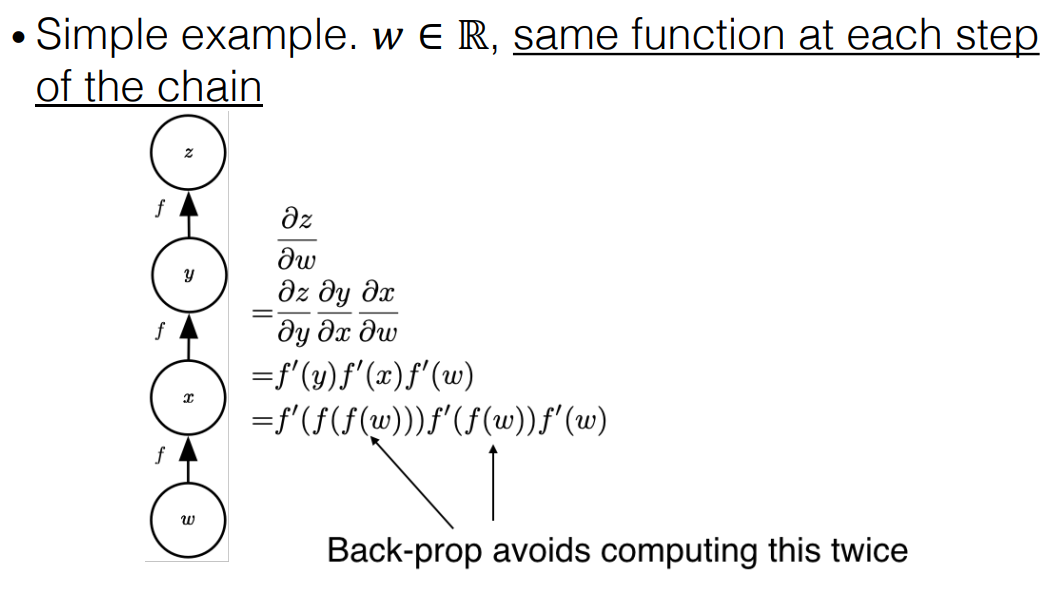
\includegraphics[scale=0.5]{images/Backprop.png}
\end{center}

\subsection{Backpropagation for (sigmoid) Perceptron}
Let's consider a Perceptron with sigmoid activation function:
\[out(\Vec{x}) = \sigma\left(\sum_{i=0}^{n} w_i x_i \right) = \sigma(\Vec{w} \cdot \Vec{x})\]
where $\sigma(net) = \frac{1}{1 + e^{-net}}$. Note that for $\sigma()$ the following relation holds:
\[\sigma'(net) = \frac{d \, \sigma(net)}{d \, net} = \sigma(net)(1 - \sigma(net))\]
Given a training set $Tr = \{(\textbf{x}^{(1)}, y^{(1)}), ..., (\textbf{x}^{(n)}, y^{(n)})\}$ and MSE cost function $E = \frac{1}{2N}\sum_{d \in Tr}(t^{(d)} - out^{(d)})^{2}$.\newline\newline
\textbf{Gradient computation for sigmoidal units:}
\begin{center}
    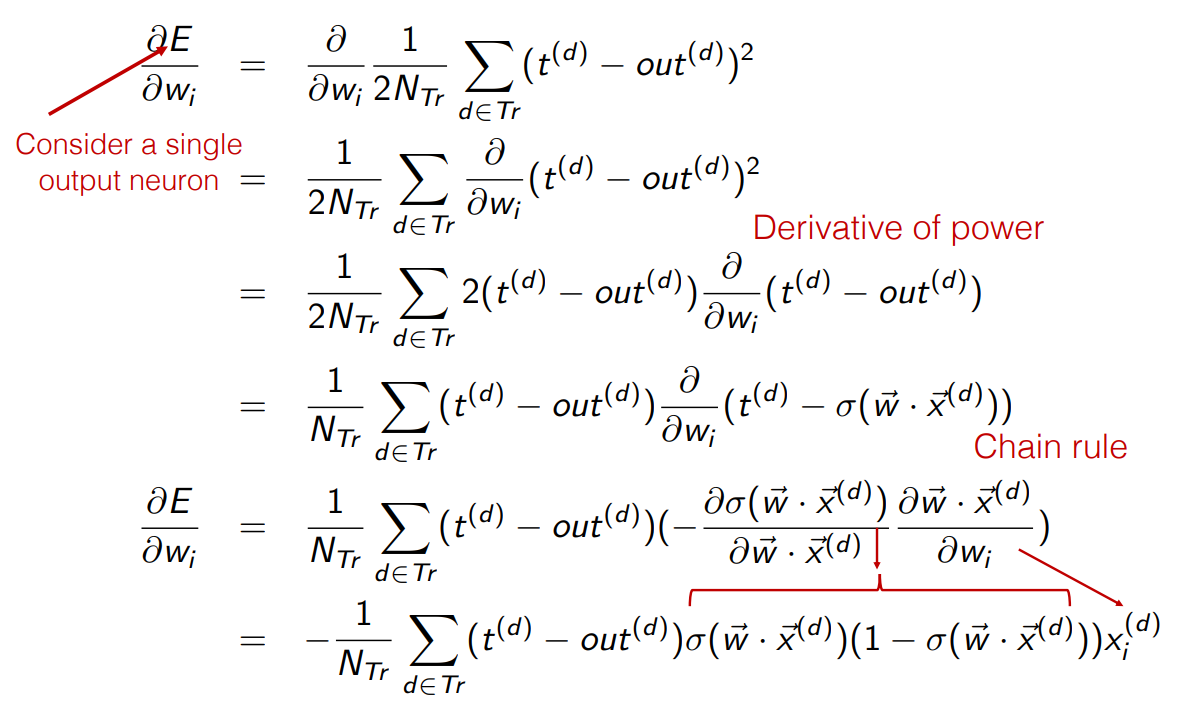
\includegraphics[scale = 0.5]{images/Derivation.png}
\end{center}

\subsection{Gradient descent for Feed-forward Networks}

Let's first define some terminology:
\begin{itemize}
    \item $d$ \textbf{input units}: $d$ input data size $\textbf{x} \equiv (x_{1},...,x_{d})$, $d + 1$ when including the bias in the weight vector $\textbf{x}^{'} \equiv (x_{0}, x_{1},...,x_{d})$

    \item $n_{H}$ \textbf{hidden units} (with output $\textbf{y} \equiv (y_{1},...,y_{n_{H}})$)

    \item $c$ \textbf{output units}: $\textbf{z} \equiv (z_{1},...,z_{c})$. The number of desired output is $\textbf{t} \equiv (t_{1},...,t_{c})$

    \item $w_{ji}$ weight from the $i$-th input unit to the $j$-th hidden unit ($w_{j}$ is the weight vector of the $j$-th hidden unit)

    \item $w_{kj}$ weight from the $j$-th hidden unit to the $k$-th output unit ($w_{k}$ is the weight vector of the $k$-th output unit)
\end{itemize}
Let's consider, for example, a Neural Network with just one hidden layer and \textbf{sigmoid activation functions}. We need to minimize an error function $E[\textbf{w}]$ that can be defined as follows:
\[E[\textbf{w}] = \frac{1}{2cN}\sum_{s=1}^{N}\sum_{k=1}^{c}(t_{k}^{(s)} - z_{k}^{(s)})^{2}\]
We need to first compute the gradient for the weights of both output and hidden units.
\begin{itemize}
    \item \textbf{Gradient of the weights of an output unit:}
    \[\frac{\partial E}{\partial w_{\hat{k}\hat{j}}} = - \frac{1}{cN}\sum_{s=1}^{N}(t_{\hat{k}}^{(s)} - z_{\hat{k}}^{(s)} )z_{\hat{k}}(1 - z_{\hat{k}})y_{\hat{j}}^{(s)}\]
    where $y_{\hat{j}}^{(s)}$ is the output of the $\hat{j}$-th hidden unit.
    
    \item \textbf{Gradient of the weights of a hidden unit:}
    \[\frac{\partial E}{\partial w_{\hat{j}\hat{i}}} = - \frac{1}{cN}\sum_{s=1}^{N}y_{\hat{j}}^{(s)}(1 - y_{\hat{j}}^{(s)})x_{\hat{i}}^{(s)}\sum_{k=1}^{c}(t_{\hat{k}}^{(s)} - z_{\hat{k}}^{(s)} )z_{\hat{k}}(1 - z_{\hat{k}})w_{k\hat{j}}\]
\end{itemize}

\textbf{Back-propagation (stochastic)}
\begin{enumerate}
    \item Initialize all weights with small random values (e.g. between -0.5 and +0.5)
    \item Until the termination condition is satisfied:
    \begin{enumerate}
        \item For each $(\textbf{x},\textbf{t}) \in S$:
        \begin{enumerate}
            \item Present $\textbf{x}$ to the net and compute the vectors $\textbf{y}$ and $\textbf{z}$
            \item For each output unit $k$:
            \[\delta_{k} = z_{k}(1 - z_{k})(t_{k} - z_{k})\]
            \[\Delta w_{kj} = \delta_{k}y_{j}\]

            \item For each hidden unit $j$:
            \[\delta_{j} = y_{j}(1 - y_{j})\sum_{k=1}^{c}w_{kj}\delta_{k}\]
            \[\Delta w_{ji} = \delta_{j}x_{i}\]

            \item Update all weights:
            \[w_{sq} \leftarrow w_{sq} + \eta \Delta w_{sq}\]
        \end{enumerate}
    \end{enumerate}
\end{enumerate}
Note that this algorithm works only for a network with one hidden layer, but can be easily extended. In fact, the algorithm computes the error term $\delta$ for each unit of each layer, and then it multiplies this error term for the input of the unit.

\section{Computational Graph}
A computational graph is a way to formalize the structure of a set of computations, such as those involved in mapping inputs and parameters to outputs and loss. Each node in the graph indicates a variable. The variable may be a scalar, vector, matrix, tensor. The edges encode operations, which are simple functions of one or more variables. Without loss of generality, we define an operation to return only a single output variable. This does not lose generality because the output variable can have multiple entries, such as a vector.\newline\newline
If a variable $y$ is computed by applying an operation to a variable $x$, then we draw a directed edge from $x$ to $y$.
\begin{center}
    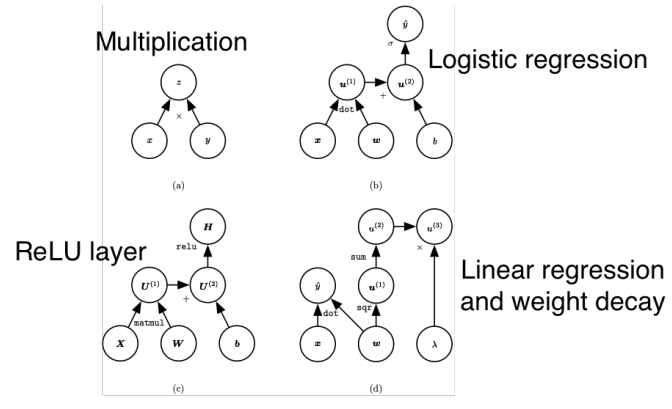
\includegraphics[scale=0.7]{images/comp graph.png}
\end{center}
